\documentclass[a4paper]{article}
\usepackage{amsfonts}
\usepackage{amsmath}
\usepackage{amssymb}
\usepackage{graphicx}     

\begin{document}
  
\noindent \large Auteur: Raj Shah \\
\noindent \large Studierichting: Informatica\\
\noindent \large Oefeningenreeks 5G nr. 7.1\\

\medskip

\normalsize

$y = x^2 , y = \dfrac{16}{x^2}, x \in [0, 4]$en $y = 0$ \\

$V_1 = \pi \displaystyle\int_{0}^{2}x^4 dx = \pi \cdot \left[\dfrac{x^5}{5}\right]_{0}^{2} = \dfrac{32\pi}{5}$\\

$V_2 = \pi \displaystyle\int_{2}^{4}\dfrac{256}{x^4}dx = 256\pi \cdot \left[\dfrac{-1}{3x^3}\right]_{2}^{4} = \dfrac{-256\pi}{192} + \dfrac{256\pi}{24}$ \\

$V_1 + V_2 = \dfrac{32\pi}{5} - \dfrac{256\pi}{192} + \dfrac{256\pi}{24}$\\

$ = \dfrac{32\pi}{5} - \dfrac{4\pi}{3} + \dfrac{32\pi}{3}$\\

$ = \dfrac{32\pi}{5} + \dfrac{28\pi}{3} = \dfrac{96\pi}{15} +\dfrac{140\pi}{15}$\\
 
$ = \dfrac{236\pi}{15}$\\

\begin{figure}[h]
\centering
    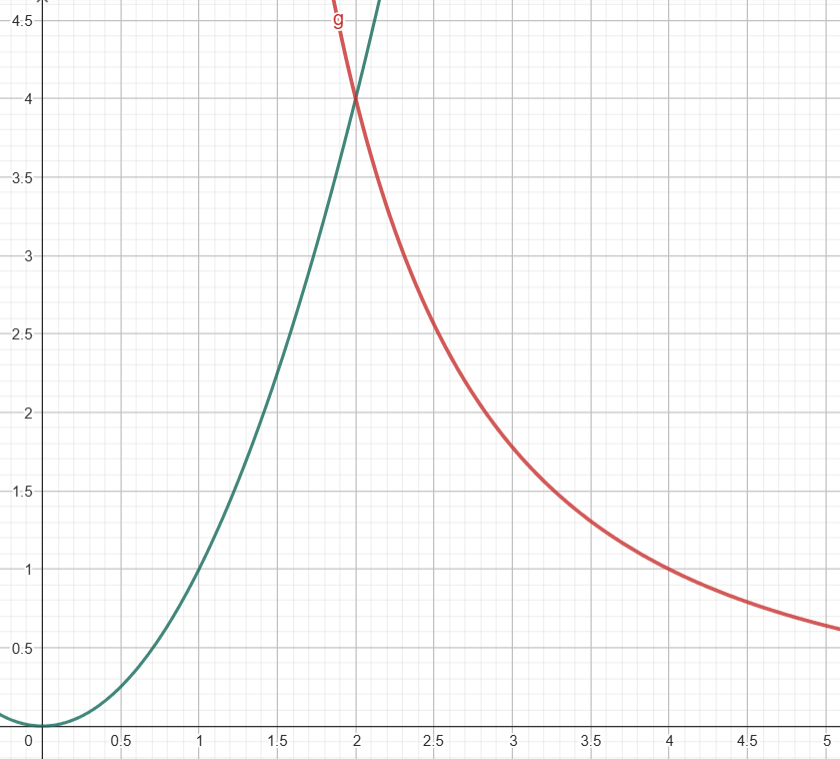
\includegraphics[width=\linewidth]{5G-7.1-raj.shah.INF.png}\\
\end{figure}

\begin{thebibliography}{999}
%\bibitem{a} Referentie
\end{thebibliography}
\end{document} 
